\chapter{Metodologia}
\label{chap:metodologia}

\section{A camada equivalente magnética e a distribuição de momentos positiva}
\label{sec:mag_eqlayer}

Seja $\Delta T(x, y, z)$ a anomalia de campo total produzida por um conjunto de fontes magnéticas no ponto $(x,y,z)$, que estão posicionadas segundo um sistema de coodenadas Cartesiano topocêntrico com os eixos $x$, $y$ e $z$ orientados para norte, leste e para baixo, respectivamente. Considere que o campo geomagético principal possua inclinação $I_{0}$ e declinação $D_{0}$ sobre a área de estudo, de forma que sua direção seja definida por um vetor unitário  

\begin{equation}
\hat{\mathbf{F}}_{0} = \begin{bmatrix}
\cos I_{0} \cos D_{0} \\
\cos I_{0} \sin D_{0} \\
\sin I_{0}
\end{bmatrix} \: .
\label{eq:campo_principal}
\end{equation}
Considere também que as fontes magnéticas tenham direção de magnetização constante definida pelo vetor unitário 

\begin{equation}
\hat{\mathbf{m}}(\mathbf{q}) = \begin{bmatrix}
\cos {I} \cos {D} \\
\cos {I} \sin {D} \\
\sin {I}
\end{bmatrix} \: ,
\label{eq:mag_vet}
\end{equation}
em que as constantes $I$ e $D$ representem a inclinação e a declinação, respectivamente, e $\mathbf{q}$ um vetor de dimensão $2 \times 1$ dado por: 

\begin{equation}
\mathbf{q} = \begin{bmatrix}
I \\ 
D
\end{bmatrix} \: .
\label{eq:q_vetor}
\end{equation}
Por conveniência, denominamos o vetor $\mathbf{q}$ como vetor de direção de magnetização. Neste caso, a anomalia de campo total $\Delta T(x, y, z)$ pode ser escrita como: 

\begin{equation}
\Delta T(x, y, z) = \, \hat{\mathbf{F}}_{0}^{\top} \mathbf{B}(x, y, z) \: 
\label{eq:tfanomaly}
\end{equation}
e $\mathbf{B}(x,y,z)$ é o campo de indução magnética dado pela equação 

\begin{equation}
\mathbf{B}(x,y,z) = \gamma_{m} \, \mathbf{M}(x, y, z) \: 
\hat{\mathbf{m}}(\mathbf{q}) \: ,
\label{eq:inducao_fonte}
\end{equation} 
em que $\gamma_{m} = 10^{-9} \frac{\mu_{0}}{4 \pi}$ (in $n \, H / m $), $\mu_{0}$ é a permeabilidade no vácuo e $\mathbf{M}(x, y, z)$ é uma matriz dada por 

\begin{equation}
	\mathbf{M}(x, y, z) = \begin{bmatrix}
		\partial_{xx} \Gamma(x, y, z) & 
		\partial_{xy} \Gamma(x, y, z) &
		\partial_{xz} \Gamma(x, y, z) \\
		\partial_{xy} \Gamma(x, y, z) & 
		\partial_{yy} \Gamma(x, y, z) &
		\partial_{yz} \Gamma(x, y, z) \\
		\partial_{xz} \Gamma(x, y, z) & 
		\partial_{yz} \Gamma(x, y, z) &
		\partial_{zz} \Gamma(x, y, z)
	\end{bmatrix} \: ,
	\label{eq:M-matrix}
\end{equation}
cujo os elementos $\partial_{\alpha\beta} \Gamma(x, y, z) \equiv 
\frac{\partial^{2} \Gamma(x, y, z)}{\partial \alpha \partial \beta}$, 
$\alpha, \beta = x, y, z$, representam as derivadas segundas da função harmônica 

\begin{equation}
\Gamma(x, y, z) = \iiint\limits_{\upsilon} 
\frac{m(x^{\prime}, y^{\prime}, z^{\prime}) \: d\upsilon^{\prime}}
{\left[ (x-x^{\prime})^2 + (y-y^{\prime})^2 + (z-z^{\prime})^2 \right]^{\frac{1}{2}}} \: .
\label{eq:Gamma-volume-integral}
\end{equation}
Nesta equação, $x^{\prime}$, $y^{\prime}$ e $z^{\prime}$ são as coordenadas do elemento de volume $d \upsilon^{\prime}$, no qual tem intensidade de magnetização $m(x^{\prime}, y^{\prime}, z^{\prime})$ (em $A/m$), localizado no interior do volume $\upsilon$ das fontes magnéticas. Consideramos que a intensidade de magnetização $m(x^{\prime}, y^{\prime}, z^{\prime})$ é estritamente positiva em todos os pontos no interior das fontes. Por conseguinte, $\Gamma(x, y, z)$ é positivo em todos os pontos exteriores a fonte magnética. Do ponto de vista físico, $\mathbf{M}(x, y, z)$ (equação \ref{eq:M-matrix}) e $\Gamma(x, y, z)$ (equação \ref{eq:Gamma-volume-integral}) representam, respectivamente, o tensor gradiente e o potencial gravitacional correspondente que seria produzido pelas fontes magnéticas no ponto $(x,y,z)$, se elas tivessem distribuição de densidade proporcional a $m(x^{\prime}, y^{\prime}, z^{\prime})$. Note que $\mathbf{M}(x, y, z)$ é uma matriz simétrica, e seu traço é zero em todos os pontos $(x,y,z)$ exteriores as fontes magnéticas e possui cinco componentes independentes que são funções harmônicas \citep{pedersen_rasmussen1990}. Explorando estas propriedades, podemos reescrever a anomalias de campo total $\Delta T(x, y, z)$ (equação \ref{eq:tfanomaly}) como uma combinação linear de cinco funções harmônicas independentes como:  

\begin{equation}
	\begin{split}
		\Delta T(x, y, z) = \:
		& a_{xx} \, \partial_{xx} \Gamma(x, y, z) + 
		a_{xy} \, \partial_{xy} \Gamma(x, y, z) + 
		a_{xz} \, \partial_{xz} \Gamma(x, y, z) + \\
		& a_{yy} \, \partial_{yy} \Gamma(x, y, z) + 
		a_{yz} \, \partial_{yz} \Gamma(x, y, z)
	\end{split} \quad ,
	\label{eq:tfanomaly-alternative}
\end{equation}
em que 

\begin{equation}
	\begin{split}
		a_{xx} &= m_{x} F_{x} - m_{z} F_{z} \\
		a_{xy} &= m_{x} F_{y} + m_{y} F_{x} \\
		a_{xz} &= m_{x} F_{z} + m_{z} F_{x} \\
		a_{yy} &= m_{y} F_{y} - m_{z} F_{z} \\
		a_{yz} &= m_{y} F_{z} + m_{z} F_{y}
	\end{split}
\label{eq:a-coefficients}
\end{equation}
são constantes definidas pelos elementos $F_{\alpha}$ e $m_{\beta}$, $\alpha = x, y, z$, $\beta = x, y, z$, dos vetores $\hat{\mathbf{F}}_{0}$ (equação \ref{eq:campo_principal}) e $\hat{\mathbf{m}}(\mathbf{q})$ (equação \ref{eq:mag_vet}), respectivamente. Por simplicidade, omitimos a dependência em relação aos parâmetros $I_{0}$ e $D_{0}$ (equação \ref{eq:campo_principal}) e $I$ e $D$ (equação \ref{eq:mag_vet}).

Seja $\Delta \tilde{T}(x, y, z)$ a anomalia de campo total produzida por uma camada contínua de dipolos que possuem direção de magnetização constante definida por um vetor unitário $\hat{\mathbf{m}}(\mathbf{q})$ (equação \ref{eq:q_vetor}), que são localizados a uma profundidade constante $z=z_c$. A anomalia de campo total produzida por esta camada fictícia pode ser definida como: 

\begin{equation}
	\Delta \tilde{T}(x, y, z) = \, \hat{\mathbf{F}}_{0}^{\top} \tilde{\mathbf{B}}(x, y, z) \: 
	\label{eq:tfanomaly-eqlayer}
\end{equation}
e $\tilde{\mathbf{B}}(x, y, z)$ é o campo de indução magnética dado por 

\begin{equation}
	\tilde{\mathbf{B}}(x, y, z) = \gamma_{m} \, \tilde{\mathbf{M}}(x, y, z) \: \hat{\mathbf{m}}(\mathbf{q}) \: ,
	\label{eq:inducao_eqlayer}
\end{equation}
em que $\tilde{\mathbf{M}}(x, y, z)$ é uma matriz dada por 

\begin{equation}
	\tilde{\mathbf{M}}(x, y, z) = \begin{bmatrix}
		\partial_{xx} \Phi(x, y, z) & 
		\partial_{xy} \Phi(x, y, z) &
		\partial_{xz} \Phi(x, y, z) \\
		\partial_{xy} \Phi(x, y, z) & 
		\partial_{yy} \Phi(x, y, z) &
		\partial_{yz} \Phi(x, y, z) \\
		\partial_{xz} \Phi(x, y, z) & 
		\partial_{yz} \Phi(x, y, z) &
		\partial_{zz} \Phi(x, y, z)
	\end{bmatrix} \quad ,
	\label{eq:M-matrix-eqlayer}
\end{equation}
com elementos $\partial_{\alpha\beta} \Phi(x, y, z) \equiv \frac{\partial^{2} \Phi(x, y, z)}{\partial \alpha \partial \beta}$, $\alpha, \beta = x, y, z$, representando as segundas derivadas da função harmônica 

\begin{equation}
	\Phi(x, y, z) = \int\limits_{-\infty}^{+\infty}\int\limits_{-\infty}^{+\infty}
	\frac{p(x'', y'', z_{c}) \: dS''}
	{\left[ (x-x'')^2 + (y-y'')^2 + (z-z_{c})^2 \right]^{\frac{1}{2}}} \: ,
	\quad z_{c} > z \: .
	\label{eq:Phi-surface-integral}
\end{equation}
Nesta equação, $x''$, $y''$ and $z_{c}$ são as coordenadas do elemento de área $dS''$, que possui momento magnético por unidade de área definido pela função $p(x'', y'', z_{c})$ (em $A$). Note que $\tilde{\mathbf{M}}(x, y, z)$ (equação \ref{eq:M-matrix-eqlayer}) também representa o tensor gradiente \citep{pedersen_rasmussen1990} e, consequentemente, simétrico possuindo traço igual a zero em todos os pontos $(x,y,z)$ acima da camada (com $z < z_{c}$) e possui cinco componentes independentes que são funções harmônicas. Estas propriedades permitem reescrever a anomalia de campo total  $\Delta \tilde{T}(x, y, z)$ (equação \ref{eq:tfanomaly-eqlayer}) como uma combinação linear de funções harmônicas dadas por

\begin{equation}
       \begin{split}
		\Delta \tilde{T}(x, y, z) = \:
		& a_{xx} \, \partial_{xx} \Phi(x, y, z) + 
		a_{xy} \, \partial_{xy} \Phi(x, y, z) + 
		a_{xz} \, \partial_{xz} \Phi(x, y, z) + \\
		& a_{yy} \, \partial_{yy} \Phi(x, y, z) + 
		a_{yz} \, \partial_{yz} \Phi(x, y, z)
		\end{split} \quad ,
	\label{eq:tfanomaly-eqlayer-alternative}
\end{equation}
com coeficientes $a_{\alpha\beta}$, $\alpha = x, y$, $\beta = x, y, z$, definidos pela equação \ref{eq:a-coefficients}.

Sabemos pela teoria do potencial que é possível encontrar uma função $p(x'', y'', z_{c})$ (equação \ref{eq:Phi-surface-integral}) na qual a condição $\Delta T(x, y, z) = \Delta \tilde{T}(x, y, z)$ é válida para todos os pontos $(x,y,z)$ localizados acima da camada fictícia de dipolos. Neste caso, a camada é chamada \textit{camada equivalente}. Para investigar tais propriedades de $p(x'', y'', z_{c})$, devemos primeiro observar que, impondo as condições acima mencionadas e utilizando as equações \ref{eq:tfanomaly-alternative} e \ref{eq:tfanomaly-eqlayer-alternative}, obtemos 

\begin{equation}
\begin{split}
a_{xx} \, &\left[\partial_{xx} \Phi(x, y, z) - \partial_{xx} \Gamma(x, y, z) \right] + \\
a_{xy} \, &\left[\partial_{xy} \Phi(x, y, z) - \partial_{xy} \Gamma(x, y, z) \right] + \\
a_{xz} \, &\left[\partial_{xz} \Phi(x, y, z) - \partial_{xz} \Gamma(x, y, z) \right] + \\
a_{yy} \, &\left[\partial_{yy} \Phi(x, y, z) - \partial_{yy} \Gamma(x, y, z) \right] + \\
a_{yz} \, &\left[\partial_{yz} \Phi(x, y, z) - \partial_{yz} \Gamma(x, y, z) \right] = 0
\: , \quad z < z_{c} \: ,
\end{split}
\label{eq:tfanomaly-alternative-equality}
\end{equation}
em que os coeficientes $a_{\alpha\beta}$ (equation \ref{eq:a-coefficients}), $\alpha = x, y$, $\beta = x, y, z$, são definidos por valores arbitrários de $I_{0}$ e $D_{0}$ (equação \ref{eq:campo_principal}) e $I$ e $D$ (equação \ref{eq:mag_vet}).

Como os coeficientes $a_{\alpha\beta}$ são não nulos, concluimos que as cinco funções harmônicas linearmente independentes devem ser zero para todos os pontos $(x,y,z)$ acima da camada equivalente, em que $z < z_{c}$. Igualando cada termo a zero e reescrevendo as segundas derivadas da integral de superfície $\Phi(x, y, z)$ (equação \ref{eq:Phi-surface-integral}), teremos 

\begin{equation}
	\partial_{\alpha\beta} \Gamma(x, y, z) = 
	\int\limits_{-\infty}^{+\infty}\int\limits_{-\infty}^{+\infty}
	p(x'', y'', z_{c}) \: \partial_{\alpha\beta} \frac{1}{r} \:\: dS'' \: ,
	\quad z_{c} > z \: ,
	\label{eq:D_alpha_beta_Gamma}
\end{equation}
em que $(x'', y'', z_{c})$ é um ponto sobre a camada equivalente e $\partial_{\alpha\beta} \frac{1}{r} \equiv \frac{\partial^{2}}{\partial \alpha \partial \beta} \frac{1}{r}$, representa a segunda derivada com respeito a  $\alpha = x, y$ e $\beta = x, y, z$, do inverso da distância da função 

\begin{equation}
   \frac{1}{r} \equiv 
	\frac{1}{\left[ (x-x'')^2 + (y-y'')^2 + (z-z_{c})^2 \right]^{\frac{1}{2}}} \: .
	\label{eq:inverse-distance}
\end{equation}
Note que a equação \ref{eq:D_alpha_beta_Gamma} é obtida derivando ambos os lados de 

\begin{equation}
\Gamma(x, y, z) = 
\int\limits_{-\infty}^{+\infty}\int\limits_{-\infty}^{+\infty}
p(x'', y'', z_{c}) \: \frac{1}{r} \:\: dS'' \: ,
\quad z_{c} > z \: .
\label{eq:Gamma_integral_equation}
\end{equation} 
Pode ser mostrado (Apêndice \ref{append:proof-positive-p}) que esta equação integral tem a solução

\begin{equation}
p(x'', y'', z_{c}) = \frac{1}{2\pi} \partial_{z} \Gamma(x'', y'', z_{c}) \: ,
\label{eq:positivity_prop}
\end{equation}
que, de acordo com a equação \ref{eq:Gamma-volume-integral}, 

\begin{equation}
\partial_{z} \Gamma(x'', y'', z_{c}) = \iiint\limits_{\upsilon} 
\frac{m(x^{\prime}, y^{\prime}, z^{\prime}) (z^{\prime} - z_{c}) \: 
d\upsilon^{\prime}}
{\left[ (x''-x^{\prime})^2 + (y''-y^{\prime})^2 + (z_{c}-z^{\prime})^2 \right]^{\frac{3}{2}}} \: , \quad z^{\prime} > z_{c} \: .
\label{eq:DzGamma-volume-integral}
\end{equation}
Do ponto de vista físico, a equação \ref{eq:DzGamma-volume-integral} representa a componente vertical da atração gravitacional (ou a pseudogravidade) que seria produzida pelas fontes magnéticas sobre a camada equivalente, se elas tivessem a distribuição de densidade proporcional a $m(x^{\prime}, y^{\prime}, z^{\prime})$. Tendo em vista que $m(x^{\prime}, y^{\prime}, z^{\prime})$ é estritamente positiva em todos os pontos $(x^{\prime}, y^{\prime}, z^{\prime})$ no interior das fontes magnéticas, $\partial_{z} \Gamma(x'', y'', z_{c})$ é positiva em todos os pontos $(x'', y'', z_{c})$ localizadas sobre a camada equivalente.

O aspecto mais interessante sobre a distribuição de momentos magnéticos $p(x'', y'', z_{c})$ (equação \ref{eq:positivity_prop}) é que ela é definida como o produto de uma constante positiva $\frac{1}{2\pi}$ e a função $\partial_{z} \Gamma(x'',y'',z_{c})$, que é estritamente positiva em todos os pontos $(x'',y'',z_{c})$ sobre a camada equivalente. Consequentemente, a função $p(x'', y'', z_{c})$ também é positiva em todos os pontos sobre a camada. Esta relação é similar àquela apresentada por \cite{pedersen1991} e \cite{li_etal_2014}. Os autores determinam, no domínio do número de onda, a distribuição de momentos magnéticos no interior de uma camada equivalente contínua com magnetização verticalmente induzida. Eles também consideram uma camada equivalente plana localizada abaixo e paralela ao plano horizontal contendo os dados observados de anomalia de campo total. Contudo, aqui não seguimos a abordagem no domínio de Fourier como estes autores. Além disso, a equação \ref{eq:positivity_prop}  generaliza a condição de positividade por que (1) é válida para todos os casos nos quais a magnetização da camada equivalente tem a mesma direção da magnetização total das fontes, mesmo que ela seja puramente induzida ou não, e (2) não requer que os dados de anomalia de campo total observados estejam em um plano.

\section{Fundamentação teórica das componentes do vetor magnético}
\label{sec:comp_vec_eqlayer}

Além do desenvolvimento matemático para a distribuição positiva de momentos magnéticos, iremos explicar teoricamente que o cálculo das componentes do vetor magnético não depende da direção de magnetização no contexto da camada equivalente. Supondo que em determinadas situações somente uma das componentes do campo de indução magnética gerado por uma rocha possa ser medida e que as medições são realizadas em regiões livres de fontes e, portanto, em pontos exteriores as rochas. Além disso, consideramos que o cálculo das componentes do vetor magnético não depende do tipo de fonte, bem como de sua configuração espacial. Assumimos também que o campo magnético não varia com o tempo, ou que esta variação seja tão pequena que pode ser desprezada ao longo das medições. Neste caso, o campo de indução magnética $\mathbf{B}(x,y,z)$ é governado pela lei de Gauss

\begin{equation}
\nabla . \mathbf{B} (x,y,z) = 0
\label{eq:gauss_B}
\end{equation}
e pela lei de Ampère 

\begin{equation}
\nabla \times \mathbf{B} (x,y,z) = 0.
\label{eq:ampere_B}
\end{equation}
Portanto, em coordenadas Cartesianas, a equação \ref{eq:ampere_B} corresponde a 

\begin{equation}
\begin{split}
\, \partial_y B_z - \partial_z B_y = 0 \:
\\
\, \partial_z B_x - \partial_x B_z = 0 \:
\\ 
\, \partial_x B_y - \partial_y B_x = 0 , 
\end{split}
\label{eq:ampere_B_condicao}
\end{equation}
em que $\partial_\alpha \equiv \dfrac{\partial}{\partial \alpha}$ é denotado como a derivada parcial em relação a coordenada $\alpha$, $\alpha=x,y,z$. 

A partir da equação \ref{eq:inducao_eqlayer}, as componentes do campo de indução magnética $\tilde{\mathbf{B}} (x,y,z)$ gerado por uma camada contínua de dipolos que tem direção de magnetização constante $\hat{\mathbf{m}} (\mathbf{q})$ posicionada a uma profundidade $z=z_c$ abaixo do plano de observação podem ser reescritas como:

\begin{equation}
\tilde{B}_{\alpha}(x, y, z) = \gamma_{m} \, \partial_{\alpha\beta} \Phi(x, y, z) m_{\beta} \: ,
\label{eq:B-eqlayer-notacao-einstein}
\end{equation}
em que $\tilde{B}_{\alpha} (x,y,z)$ é a componente $\alpha$, $\alpha=x,y,z$, do campo de indução magnética e $m_{\beta}$ é a componente $\beta$, $\beta =x,y,z$, da direção de magnetização $\hat{\mathbf{m}} (\mathbf{q})$ da camada. Por conveniência, a componente vertical do campo magnético pode ser escrita como:  

\begin{equation}
\tilde{B}_{z}(x, y, z) = \gamma_{m} \,[ \partial_{xz} \Phi^{\dagger}(x, y, z) m_{x}^{\dagger} + \partial_{yz} \Phi^{\dagger}(x, y, z) m_{y}^{\dagger} + \partial_{zz} \Phi^{\dagger}(x, y, z) m_{z}^{\dagger} ]  \: ,
\label{eq:Bz-eqlayer}
\end{equation}
em que a função harmônica $\Phi^{\dagger}(x, y, z)$ é dada por 

\begin{equation}
\Phi^{\dagger}(x, y, z) = \int\limits_{-\infty}^{+\infty}\int\limits_{-\infty}^{+\infty}
\frac{p^{\dagger}(x'', y'', z_{c}) \: dS''}
{\left[ (x-x'')^2 + (y-y'')^2 + (z-z_{c})^2 \right]^{\frac{1}{2}}} \: .
\label{eq:Phi-integral-superficie-Bz}
\end{equation}
A função $p^{\dagger}(x'', y'', z_{c})$ descreve a distribuição de momentos magnéticos por unidade de área relativa a componente $\tilde{B}_{z}(x, y, z)$ do campo de indução magnética gerado por uma camada contínua e direção de magnetização $\hat{\mathbf{m}}^{\dagger}(\mathbf{q})$ que possui componentes $m_{\beta}^{\dagger}$, $\beta = x,y,z$. Analogamente, podemos escrever as outras duas componentes do campo como:

\begin{equation}
\tilde{B}_{x}(x, y, z) = \gamma_{m} \, [\partial_{xx} \Phi^{\ddagger}(x, y, z) m_{x}^{\ddagger} + \partial_{xy} \Phi^{\ddagger}(x, y, z) m_{y}^{\ddagger} + \partial_{xz} \Phi^{\ddagger}(x, y, z) m_{z}^{\ddagger}]   \: 
\label{eq:Bx-eqlayer}
\end{equation}
e 

\begin{equation}
\tilde{B}_{y}(x, y, z) = \gamma_{m} \, [\partial_{xy} \Phi^{\sharp}(x, y, z) m_{x}^{\sharp} + \partial_{yy} \Phi^{\sharp}(x, y, z) m_{y}^{\sharp} + \partial_{yz} \Phi^{\sharp}(x, y, z) m_{z}^{\sharp}]   \: ,
\label{eq:By-eqlayer}
\end{equation}
em que $\tilde{B}_{x} (x,y,z)$ e $\tilde{B}_{y} (x,y,z)$ são as componentes do campo magnético que dependem das funcões harmônicas $\Phi^{\ddagger}(x, y, z)$ e $\Phi^{\sharp}(x, y, z)$ e das direções de magnetização $\hat{\mathbf{m}}^{\ddagger}(\mathbf{q})$ e $\hat{\mathbf{m}}^{\sharp}(\mathbf{q})$, respectivamente. Note que as equações \ref{eq:Bz-eqlayer}, \ref{eq:Bx-eqlayer} e \ref{eq:By-eqlayer} representam as camadas contínuas que geram as componentes do vetor magnético com suas respectivas direções magnetização e distribuições de momentos magnéticos. 

Aplicando as condições de contorno acima mencionadas pelas equações \ref{eq:ampere_B_condicao} nas componentes do vetor magnético teremos que

\begin{equation}
\begin{split}
&[\partial_{xyz} \Phi^{\dagger}(x, y, z) m_{x}^{\dagger} - \partial_{xyz} \Phi^{\sharp}(x, y, z) m_{x}^{\sharp}] + \:
\\ 
&[\partial_{xyy} \Phi^{\dagger}(x, y, z) m_{y}^{\dagger} - \partial_{xyy} \Phi^{\sharp}(x, y, z) m_{y}^{\sharp}] + \:
\\ 
&[\partial_{xyz} \Phi^{\dagger}(x, y, z) m_{z}^{\dagger} - \partial_{xyz} \Phi^{\sharp}(x, y, z) m_{z}^{\sharp}] = 0,
\end{split}
\label{eq:condicoes_equacao1}
\end{equation}

\begin{equation}
\begin{split}
&[\partial_{xxz} \Phi^{\ddagger}(x, y, z) m_{x}^{\ddagger} - \partial_{xxz} \Phi^{\dagger}(x, y, z) m_{x}^{\dagger}] + 
\\ 
&[\partial_{xyz} \Phi^{\ddagger}(x, y, z) m_{y}^{\ddagger} - \partial_{xyz} \Phi^{\dagger}(x, y, z) m_{y}^{\dagger}] + 
\\ 
&[\partial_{xzz} \Phi^{\ddagger}(x, y, z) m_{z}^{\ddagger} - \partial_{xzz} \Phi^{\dagger}(x, y, z) m_{z}^{\dagger}]= 0 
\end{split}
\label{eq:condicoes_equacao2}
\end{equation}
e

\begin{equation}
\begin{split}
&[\partial_{xxy} \Phi^{\sharp}(x, y, z) m_{x}^{\sharp} - \partial_{xxy} \Phi^{\ddagger}(x, y, z) m_{x}^{\ddagger}] + 
\\ 
&[\partial_{xyz} \Phi^{\sharp}(x, y, z) m_{y}^{\sharp} - \partial_{xyz} \Phi^{\ddagger}(x, y, z) m_{y}^{\ddagger}] + 
\\
&[\partial_{xzz} \Phi^{\sharp}(x, y, z) m_{z}^{\sharp} - \partial_{xzz} \Phi^{\ddagger}(x, y, z) m_{z}^{\ddagger}]  = 0.
\end{split}
\label{eq:condicoes_equacao3}
\end{equation}
Note que para satisfazer as condições apresentadas pelas equações \ref{eq:ampere_B_condicao} e de acordo com as equações \ref{eq:condicoes_equacao1}, \ref{eq:condicoes_equacao2} e \ref{eq:condicoes_equacao3}, as distribuições de momentos magnéticos e as direções de magnetização das camadas que ajustam as componentes do vetor de indução magnética devem ser iguais. Portanto, isto nos leva que 

\begin{equation}
p^{\dagger}(x'', y'', z_{c}) = p^{\ddagger}(x'', y'', z_{c}) = p^{\sharp}(x'', y'', z_{c})
\label{eq:momentos_iguais}
\end{equation}
e 

\begin{equation}
\begin{split}
&m_{x}^{\dagger} = m_{x}^{\ddagger} = m_{x}^{\sharp} 
\\
&m_{y}^{\dagger} = m_{y}^{\ddagger} = m_{y}^{\sharp} 
\\
&m_{z}^{\dagger} = m_{z}^{\ddagger} = m_{z}^{\sharp}.
\end{split}
\label{eq:direcoes_iguais}
\end{equation}
O que as equações \ref{eq:momentos_iguais} e \ref{eq:direcoes_iguais} nos diz é que uma vez que conheçamos a distribuição de momentos magnéticos e a direção de magnetização que ajustam uma das componentes conseguimos recuperar as outras duas. Além disso, as derivadas parciais $\partial_{\alpha\beta} \Phi(x, y, z)$, $\alpha, \beta = x, y, z$ são tomadas em relação a $x$, $y$ e $z$ das funções harmônicas, fazendo com que todo o cálculo das componentes do vetor magnético não dependa das componentes $m_\beta$, $\beta = x,y,z$, da direção de magnetização. Portanto, é possível ajustar todas as componentes do vetor magnético a partir de uma distribuição de momentos magnéticos associada a qualquer direção de magnetização arbitrária imposta sobre a camada.  
 
%%% Discretizing layer
\section{Parametrização e o problema direto}
\label{sec:par_prob_dir}

\subsection{Para a anomalia de campo total}
\label{subsec:tf_prob_dir}

Em situações práticas, não é possível determinar uma distribuição contínua de momentos magnéticos $p(x'',y'',z_{c})$ (equação \ref{eq:positivity_prop}) sobre a camada equivalente. Por esta razão, a camada tem que ser aproximada por um conjunto discreto de dipolos (fontes equivalentes) de volume unitário localizado a uma profundidade constante e igual a $z = z_c$ (Figura \ref{fig:eqlayer_tfa_sketch}). A anomalia de campo total produzida por esta camada discreta (anomalia de campo total predita) no ponto $(x_i,y_i,z_i)$, $i=1,\dots,N$, é dada por 

\begin{equation}
\Delta T_{i}(\mathbf{s}) = \mathbf{g}_{i}(\mathbf{q})^{\top} \mathbf{p},
\label{eq:tfa_pred_i}
\end{equation}
em que $\mathbf{s}$ é um vetor $(M + 2) \times 1$ particionado (vetor de dados preditos) dado por 

\begin{equation}
      \mathbf{s} = \begin{bmatrix}
		\mathbf{p} \\
		\mathbf{q}
	\end{bmatrix} \: ,
	\label{eq:parameter-vector}
\end{equation}
$\mathbf{q}$ é o vetor direção de magnetização (equação \ref{eq:q_vetor}), $\mathbf{p}$ é um vetor $M \times 1$ (vetor de momentos magnéticos) cujo $j$-ésimo elemento, $j=1,\dots,M$, é a intensidade do momento magnético $p_{j}$ (em $A \, m^{2}$) dos $j$-ésimo dipolo e $\mathbf{g}_{i} (\mathbf{q})$ é outro vetor $M \times 1$ cujo $j$-ésimo elemento é definido pela função harmônica 

\begin{equation}
g_{ij} (\mathbf{q})  = \gamma_m \hat{\mathbf{F}}_{0}^T \, 
\mathbf{M}_{ij} \, \hat{\mathbf{m}}(\mathbf{q}) \: .
\label{eq:g_ij}
\end{equation}
Nesta equação, $\mathbf{M}_{ij}$ é uma matriz $3 \times 3$ dada por 

\begin{equation}
\mathbf{M}_{ij} = \begin{bmatrix}
\partial_{xx} \frac{1}{r} & 
\partial_{xy} \frac{1}{r} &
\partial_{xz} \frac{1}{r} \\
\partial_{xy} \frac{1}{r} & 
\partial_{yy} \frac{1}{r} &
\partial_{yz} \frac{1}{r} \\
\partial_{xz} \frac{1}{r} & 
\partial_{yz} \frac{1}{r} &
\partial_{zz} \frac{1}{r}
\end{bmatrix} \quad ,
\label{eq:Mij-matrix}
\end{equation}
em que $\partial_{\alpha\beta} \frac{1}{r} \equiv \frac{\partial^{2}}{\partial \alpha \partial \beta} \frac{1}{r}$, representa a derivada segunda com respeito a $\alpha = x, y, z$ e $\beta = x, y, z$, do inverso da distância $\frac{1}{r}$ (equação \ref{eq:inverse-distance}) entre as coordenadas de observação $(x, y, z) = (x_{i}, y_{i}, z_{i})$ e as coordenadas das fontes equivalentes $(x'', y'', z_{c}) = (x_{j}, y_{j}, z_{c})$. As equações $\ref{eq:tfa_pred_i}$-$\ref{eq:Mij-matrix}$ mostram que a anomalia de campo total predita $\Delta T_{i}(\mathbf{s})$ possui uma relação linear com o vetor de momentos magnéticos $\mathbf{p}$ e uma relação não linear com o vetor de direção de magnetização $\mathbf{q}$ (equação \ref{eq:q_vetor}).

%% Figura 

\begin{figure}[H]
	\centering
	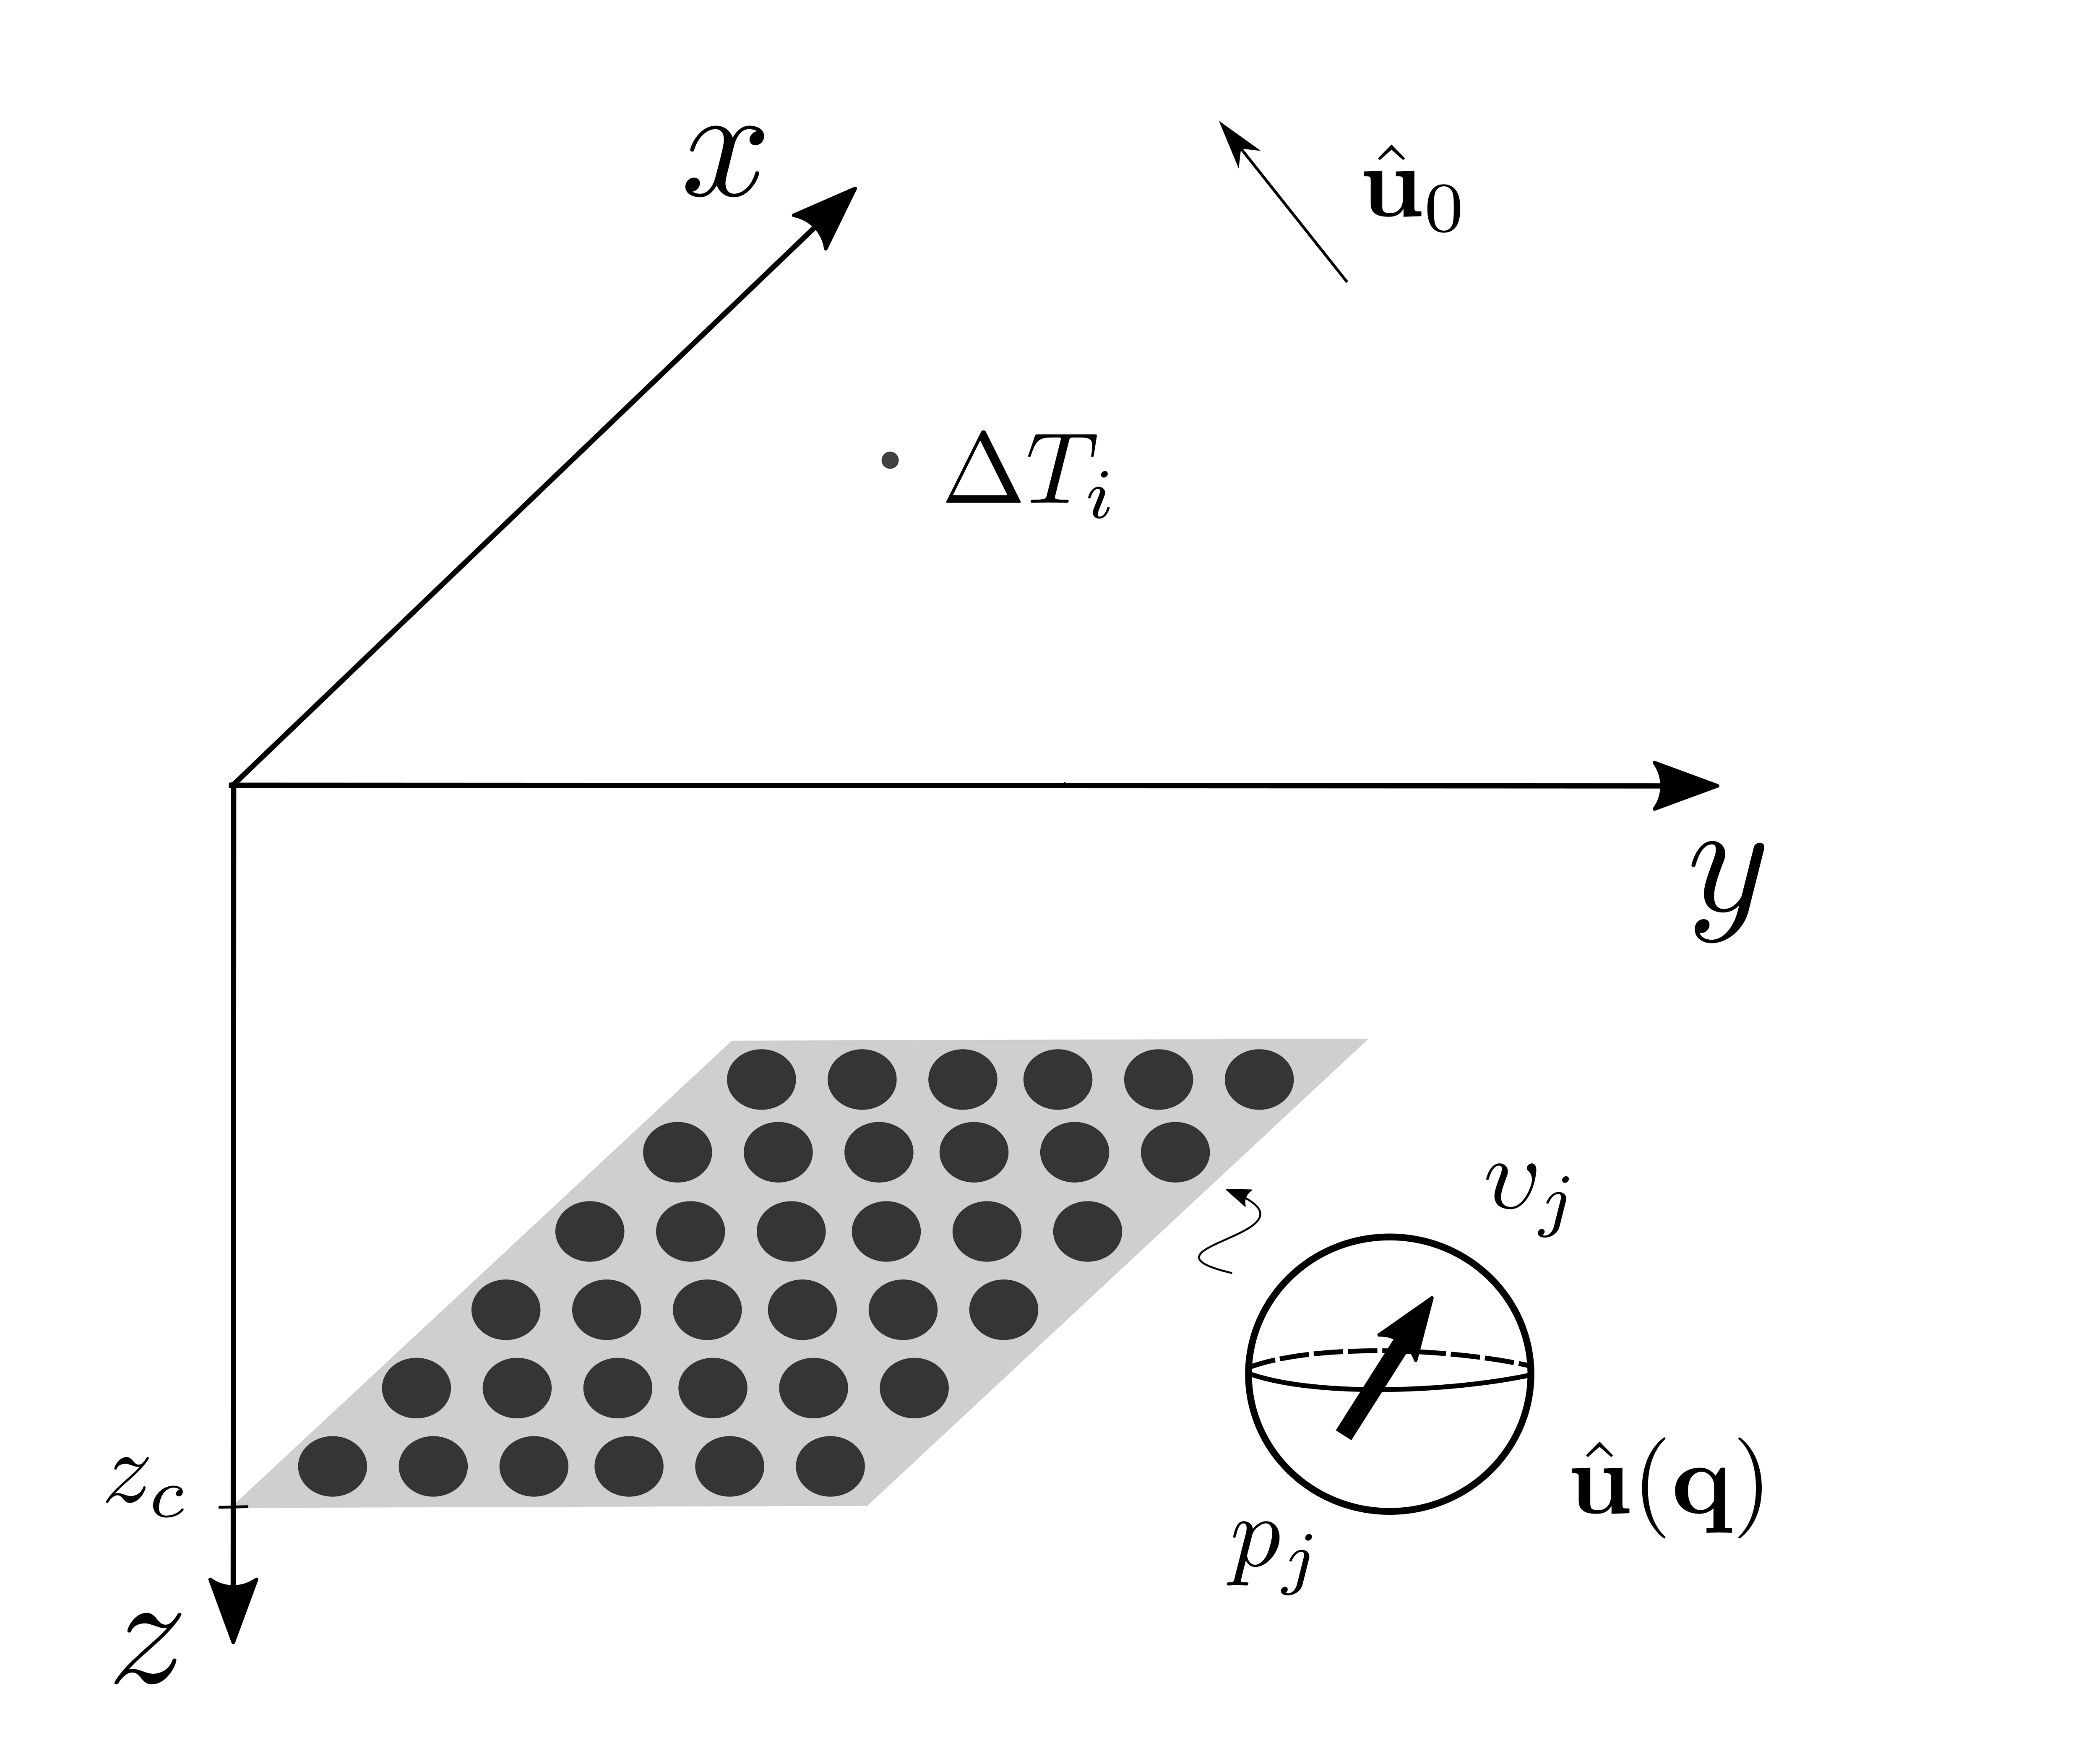
\includegraphics[width=.7\textwidth]{Fig/eqlayer/eqlayer_figure_tfa.png}
	\caption{Representação esquemática da camada equivalente para a anomalia de campo total. A camada é posicionada sobre o plano horizontal a uma profundidade $z=z_c$. $\Delta T_i$ é a anomalia de campo total predita no ponto $(x_i,y_i,z_i)$ produzida pelo conjunto de $M$ fontes equivalentes (pontos pretos). Cada fonte é localizada no ponto  $(x_j,y_j,z_c)$, $j = 1,\hdots, M$, e são representadas por um dipolo de volume unitário $\upsilon$ com direção de magnetização $\hat{\mathbf{m}}(\mathbf{q})$ e momento magnético $p_j$. $\hat{\mathbf{F}}_{0}$ é um vetor unitário na direção do campo geomagnético.}
	\label{fig:eqlayer_tfa_sketch}
\end{figure}

\subsection{Para a componente vertical do campo magnético}
\label{subsec:bz_prob_dir}

De forma análoga a seção \ref{subsec:tf_prob_dir}, a componente vertical do campo de indução magnética (componente vertical predita) produzida por uma camada discreta posicionada a uma profundidade constante $z=z_c$ no ponto $(x_i,y_i,z_i)$, $i=1,\dots,N$, (Figura \ref{fig:eqlayer_bz_sketch}) é dada por 

\begin{equation}
B_{zi} (\mathbf{s})  = \mathbf{g}_{i}^{z}(\mathbf{q})^{\top} \, \mathbf{p},
\label{eq:pred_data_ith-z}
\end{equation}
em que $\mathbf{s}$ é um vetor $(M + 2) \times 1$ particionado (vetor de dados preditos) dado por 

\begin{equation}
      \mathbf{s} = \begin{bmatrix}
		\mathbf{p} \\
		\mathbf{q}
	\end{bmatrix} \: ,
	\label{eq:parameter-vector-z}
\end{equation}
$\mathbf{q}$ é o vetor direção de magnetização (equação \ref{eq:q_vetor}), $\mathbf{p}$ é um vetor $M \times 1$ (vetor de momentos magnéticos) cujo $j$-ésimo elemento, $j=1,\dots,M$, é a intensidade do momento magnético $p_{j}$ (em $A \, m^{2}$) dos $j$-ésimo dipolo e $\mathbf{g}_{i}^{z} (\mathbf{q})$ é outro vetor $M \times 1$ cujo $j$-ésimo elemento é definido pela função harmônica 

\begin{equation}
g_{ij}^{z}(\mathbf{q})  = \gamma_m \, \mathbf{M}_{ij}^{z^\top} \, \hat{\mathbf{m}}(\mathbf{q}) \: .
\label{eq:g_ij-z}
\end{equation}
Nesta equação, $\mathbf{M}_{ij}^{z^\top}$ é um vetor $1 \times 3$ dada por 

\begin{equation}
\mathbf{M}_{ij}^{z^\top} = \begin{bmatrix}
\partial_{xz} \frac{1}{r} & 
\partial_{yz} \frac{1}{r} &
\partial_{zz} \frac{1}{r}
\end{bmatrix}^\top \quad ,
\label{eq:Mij-matrix-z}
\end{equation}
em que $\partial_{\alpha z} \frac{1}{r} \equiv \frac{\partial^{2}}{\partial \alpha \partial z} \frac{1}{r}$, representa a derivada segunda com respeito a $\alpha = x, y, z$, do inverso da distância $\frac{1}{r}$ (equação \ref{eq:inverse-distance}) entre as coordenadas de observação $(x, y, z) = (x_{i}, y_{i}, z_{i})$ e as coordenadas das fontes equivalentes $(x'', y'', z_{c}) = (x_{j}, y_{j}, z_{c})$. Note que, analogamente a seção \ref{subsec:tf_prob_dir}, a componente vertical do campo $B_{zi}(\mathbf{s})$ possui uma relação linear com o vetor de momentos magnéticos $\mathbf{p}$ e uma relação não linear com o vetor de direção de magnetização $\mathbf{q}$ (equação \ref{eq:q_vetor}).

%% Figura
\begin{figure}[H]
	\centering
	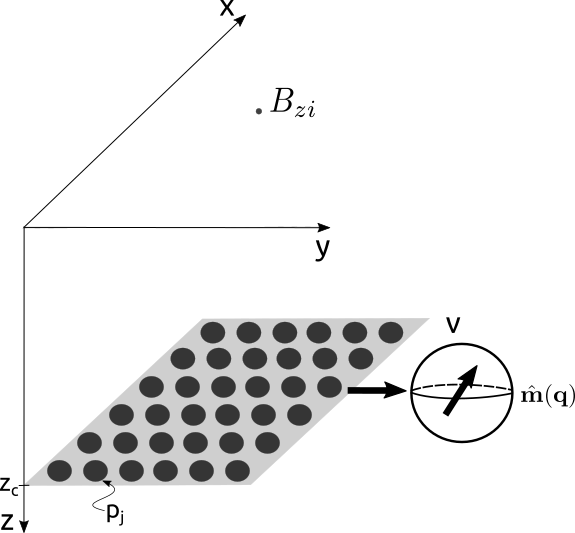
\includegraphics[width=.7\textwidth]{Fig/mag_vec/eqlayer_figure_bz.png}
	\caption{Representação esquemática da camada equivalente para a componente vertical do campo magnético. A camada também é posicionada sobre o plano horizontal a uma profundidade $z=z_c$, de forma similar para a anomalia de campo total (Figura \ref{fig:eqlayer_tfa_sketch}). $B_{zi}$ é a componente vertical do campo magnético predita no ponto $(x_i,y_i,z_i)$ produzida pelo conjunto de $M$ fontes equivalentes (pontos pretos). Cada fonte é localizada no ponto  $(x_j,y_j,z_c)$, $j = 1,\hdots, M$, e são representadas por um dipolo de volume unitário $\upsilon$ com direção de magnetização $\hat{\mathbf{m}}(\mathbf{q})$ e momento magnético $p_j$.}
	\label{fig:eqlayer_bz_sketch}
\end{figure}


\section{Problema inverso}

\subsection{A estimativa da direção de magnetização}
\label{subsec:mag_dir_est}

%%%%% Defining the objective function
Seja $\mathbf{\Delta T}^{o}$ o vetor de dados observados cujo $i$-ésimo elemento $\Delta T_{i}^{o}$ é a anomalia de campo total produzida por uma fonte magnética no ponto $(x_{i},y_{i},z_{i})$, $i = 1, \dots, N$. Similarmente, seja $\mathbf{\Delta T} (\mathbf{s})$ o vetor de dados preditos cujo $i$-ésimo elemento $\Delta T_{i}(\mathbf{s})$ (equação \ref{eq:tfa_pred_i}) é a anomalia de campo total produzida por uma camada equivalente discreta no mesmo ponto $(x_{i},y_{i},z_{i})$. Com o objetivo de estimarmos um vetor de parâmetros $\mathbf{s}$ (equação \ref{eq:parameter-vector}) que minimiza a diferença entre $\mathbf{\Delta T}^{o}$ e $\mathbf{\Delta T}(\mathbf{s})$, temos que resolver o problema inverso:

\begin{subequations}
	\begin{align}
	& \text{minimizar}
	& &\Psi(\mathbf{s}) =\lVert \mathbf{\Delta T}^{o} - \mathbf{\Delta T} (\mathbf{s}) 
	\rVert_{2}^{2} + \, \mu f_0 \parallel \mathbf{p} \parallel_{2}^{2} \: , \\
	& \text{sujeito a}
	& & \mathbf{p} \geqslant \mathbf{0} \: .
	\end{align}
	\label{eq:positivity_goal_function}
\end{subequations}
O primeiro e o segundo termo da equação \ref{eq:positivity_goal_function}a são, respectivamente, a função de ajuste e a função regularizadora de Tikhonov de ordem zero, $\mu$ é o parâmetro de regularização, $\| \cdot \|_{2}^{2}$ representa o quadrado da norma Euclidiana e $f_{0}$ é um fator de normalização. Na inequação \ref{eq:positivity_goal_function}b, $\mathbf{0}$ é um vetor $M \times 1$ com todos os elementos iguais a zero no qual o sinal da inequação é aplicado elemento a elemento. Este vínculo de positividade sobre o vetor de momentos magnéticos $\mathbf{p}$ é incorporado utilizando o chamado \textit{estimador de mínimos quadrados não negativo} ou somente NNLS (do inglês \textit{Nonnegative least squares}) proposto por \cite{lawson_hanson_1974}.

Para resolver este problema inverso, temos que considerar primeiramente uma expansão até segunda ordem da função objetivo (equação \ref{eq:positivity_goal_function}a) em torno de $\mathbf{s} = \mathbf{s}^{k}$ (equação \ref{eq:parameter-vector}):

\begin{equation}
\Psi(\mathbf{s}^{k} + \mathbf{\Delta s}^{k}) \approx \Psi(\mathbf{s}^{k}) + 
{\mathbf{J}^{k}}^{\top} \mathbf{\Delta s}^{k} + 
\frac{1}{2} {\mathbf{\Delta s}^{k}}^{\top} \mathbf{H}^{k} \mathbf{\Delta s}^{k}  \: ,
\label{eq:sec_ord_goal}
\end{equation}
em que $\mathbf{\Delta s}^{k}$ é uma perturbação no vetor de parâmetros e os termos $\mathbf{J}^{k}$ e $\mathbf{H}^{k}$ são, respectivamente, o vetor gradiente e a matriz Hessiana avaliadas em $\mathbf{s}^{k}$. Então, estimamos o vetor de perturbação $\bar{\mathbf{\Delta s}}^k$ que minimiza a função expandida (equação \ref{eq:sec_ord_goal}) tomando o seu gradiente e igualando o resultado ao vetor nulo. Este procedimento nos leva ao sistema linear 

\begin{equation}
\mathbf{H}^{k} \bar{\mathbf{\Delta s}}^{k} = - \mathbf{J}^{k} \: ,
\label{eq:linear_sys_GN}
\end{equation}
que representa o $k$-ésimo passo do método de Gauss-Newton \citep{aster2005} para a minimização da função objetivo (equação \ref{eq:positivity_goal_function}a). Reescrevemos este sistema linear desprezando as derivadas cruzadas na matriz Hessiana como: 

\begin{equation}
\left[
\begin{array}{c|c}
\mathbf{H}_{pp}^{k} & \mathbf{0} \\
\hline
\mathbf{0}^{\top} & \mathbf{H}_{qq}^{k}
\end{array}
\right] \left[ \begin{array}{c}
\bar{\mathbf{\Delta p}}^{k} \\ 
\bar{\mathbf{\Delta q}}^{k} 
\end{array} \right] \approx -\left[ \begin{array}{c}
\mathbf{J}_{p}^{k} \\ 
\mathbf{J}_{q}^{k} 
\end{array} \right] ,
\label{eq:linear_sys_GN_block}
\end{equation}
em que $\mathbf{0}$ é uma matriz $M \times 2$ que contém todos os elementos iguais a zero, $\bar{\mathbf{\Delta p}}^{k} = \bar{\mathbf{p}}^{k+1} - \bar{\mathbf{p}}^{k}$ é a correção no vetor de momentos magnéticos $\mathbf{p}$, $\bar{\mathbf{\Delta q}}^{k} = \bar{\mathbf{q}}^{k+1} - \bar{\mathbf{q}}^{k}$ é a correção no vetor direção de magnetização e os termos $\mathbf{J}_{\alpha}^{k}$ e $\mathbf{H}_{\alpha \alpha}^{k}$, $\alpha = p,q$, são os vetores gradientes e as matrizes Hessianas calculadas com respeito aos elementos dos $\mathbf{p}$ e $\mathbf{q}$, respectivamente. 

O vetor gradiente $\mathbf{J}_{p}^{k}$ e a matriz Hessiana $\mathbf{H}_{pp}^{k}$ (equação \ref{eq:linear_sys_GN_block}) relativas ao vetor de momentos magnéticos $\mathbf{p}$ (equação \ref{eq:parameter-vector}) são, respectivamente, 

\begin{equation}
\mathbf{J}_{p}^{k} = -2 {\mathbf{G}_{p}^{k}}^{\top} 
\left[ \mathbf{\Delta T}^{o} - \mathbf{\Delta T} (\bar{\mathbf{s}}^{k}) \right] + 
2\mu f_{0}^{k} \bar{\mathbf{p}}^{k} 
\label{eq:grad_p}
\end{equation}
e 

\begin{equation}
\mathbf{H}_{pp}^{k} = 2 {\mathbf{G}_{p}^{k}}^{\top} \mathbf{G}_{p}^{k} + 
2 \mu f_{0}^{k} \mathbf{I} \: ,
\label{eq:hess_p}
\end{equation}
em que $\mathbf{G}_p^{k}$ é uma matriz de dimensão $N \times M$ cujo $ij$-ésimo elemento é dado pela função harmônica $g_{ij}(\bar{\mathbf{q}}^{k})$ (equação \ref{eq:g_ij}) avaliada na direção de magnetização $\bar{\mathbf{q}}^{k}$, $\mathbf{I}$ é uma matriz identidade de dimensão $M \times M$ e $f_{0}^{k}$ é um fator de normalização igual a 

\begin{equation}
f_{0}^{k} = \dfrac{trace \left({\mathbf{G}_{p}^{k}}^{\top} \mathbf{G}_{p}^{k} \right)}{M} \, .
\label{eq:norm_factor}
\end{equation}

O vetor gradiente $\mathbf{J}_{q}^{k}$ e a matriz Hessiana $\mathbf{H}_{qq}^{k}$ (equação \ref{eq:linear_sys_GN_block}) relativas a direção de magnetização $\mathbf{q}$ (equação \ref{eq:q_vetor}) são, respectivamente, 

\begin{equation}
\mathbf{J}_{q}^{k} = -2 {\mathbf{G}_{q}^{k}}^{\top} 
\left[ \mathbf{\Delta T}^{o} - \mathbf{\Delta T} (\bar{\mathbf{s}}^{k}) \right]
\label{eq:grad_q}
\end{equation}
e

\begin{equation}
\mathbf{H}_{qq}^{k} \approx 2 {\mathbf{G}_{q}^{k}}{^\top} \mathbf{G}_{q}^{k} \: ,
\label{eq:hess_q}
\end{equation}
em que $\mathbf{G}_{q}^{k}$ é uma matriz $N \times 2$ dada por 

\begin{equation}
\mathbf{G}_{q}^{k} = \begin{bmatrix}
\partial_{I} \mathbf{g}_{1}(\bar{\mathbf{q}}^{k})^{\top} \bar{\mathbf{p}}^{k} & 
\partial_{D} \mathbf{g}_{1}(\bar{\mathbf{q}}^{k})^{\top} \bar{\mathbf{p}}^{k} \\
\vdots & \vdots  \\
\partial_{I} \mathbf{g}_{N}(\bar{\mathbf{q}}^{k})^{\top} \bar{\mathbf{p}}^{k} & 
\partial_{D} \mathbf{g}_{N}(\bar{\mathbf{q}}^{k})^{\top} \bar{\mathbf{p}}^{k} 
\end{bmatrix} \: ,
\label{eq:Gq}
\end{equation}
em que $\partial_{\alpha} \mathbf{g}_{i}(\bar{\mathbf{q}}^{k}) \equiv \frac{\partial \mathbf{g}_{i}(\bar{\mathbf{q}}^{k})}{\partial \alpha}$, $\alpha= I, D$, representa a primeira derivada do vetor $\mathbf{g}_{i}(\bar{\mathbf{q}}^{k})$ (equação \ref{eq:tfa_pred_i}) com respeito a inclinação $I$ e a declinação $D$ da magnetização total das fontes.

\subsubsection{Processo iterativo para a estimativa da direção de magnetização}

A iteração $k=0$ do nosso algoritmo começa com uma aproximação inicial $\bar{\mathbf{q}}^{k} = \bar{\mathbf{q}}^{0}$ para o vetor direção de magnetização $\mathbf{q}$ (equação \ref{eq:q_vetor}). Utilizando esta aproximação inicial $\bar{\mathbf{q}}^{k}$, a parte superior da equação \ref{eq:linear_sys_GN_block} nos leva ao seguinte sistema linear para o vetor de momentos magnéticos:

\begin{equation}
\left[ {\mathbf{G}_{p}^{k}}^{\top} \mathbf{G}_{p}^{k} + 
\mu f_{0}^{k} \mathbf{I} \right] \bar{\mathbf{p}}^{k} = {\mathbf{G}_{p}^{k}}^{\top} \mathbf{\Delta T}^{o} \: .
\label{eq:linear_sys_p}
\end{equation}
Para impor o vínculo de positividade (equação \ref{eq:positivity_goal_function}b) sobre a distribuição de momentos magnéticos, este sistema linear é resolvido usando o método de NNLS \citep{lawson_hanson_1974, silvadias_etal_2010}. Esta distribuição de momentos magnéticos é então usada para estimar uma correção $\bar{\mathbf{\Delta q}}^{k}$ no vetor direção de magnetização resolvendo um sistema não linear utilizando o método de Levenberg-Marquardt \citep{aster2005}:

\begin{equation}
\left[ {\mathbf{G}_{q}^{k}}^{\top} \mathbf{G}_{q}^{k} + \lambda \, \mathbf{I} \right] 
\bar{\mathbf{\Delta q}}^{k} = {\mathbf{G}_{q}^{k}}^{\top} 
\left[ \mathbf{\Delta T}^{o} - \mathbf{\Delta T} (\mathbf{s}^{k}) \right] \: ,
\label{eq:linear_sys_q}
\end{equation}
em que $\lambda$ é o parâmetro de Marquardt e $\mathbf{I}$ é uma matriz identidade. Após estimarmos a correção $\bar{\mathbf{\Delta q}}^{k}$ na $k$-ésima iteração, atualizamos a direção de magnetização aplicando a correção a seguir:

\begin{equation}
\bar{\mathbf{q}}^{k+1} = \bar{\mathbf{q}}^{k} + \bar{\mathbf{\Delta q}}^{k} \: ,
\label{eq:q_next}
\end{equation}
e utilizando esta nova direção para estimar uma nova distribuição de momentos magnéticos com a equação \ref{eq:linear_sys_p} e assim sucessivamente. O processo iterativo é interrompido quando a função objetivo (equação \ref{eq:positivity_goal_function}a) é invariante ao longo de sucessivas iterações. Mostramos também que este método falha em situações nas quais as fontes são magnetizadas verticalmente (Apêndice \ref{append:vertical-magnetization}).

\subsection{O cálculo das componentes do campo magnético e a amplitude do campo}
\label{subsec:componentes_vec}

Seja $\mathbf{B}_{z}^{o}$ o vetor de dados observados cujo $i$-ésimo elemento $B_{zi}^{o}$ é a componente vertical do campo magnético produzida por uma fonte magnética no ponto $(x_{i},y_{i},z_{i})$, $i = 1, \dots, N$. Similarmente, seja $\mathbf{B}_{z}^{p} (\mathbf{s})$ o vetor de dados preditos cujo $i$-ésimo elemento $B_{zi}^{p}(\mathbf{s})$ (equação \ref{eq:pred_data_ith-z}) é a componente vertical do campo magnético produzida por uma camada equivalente discreta no mesmo ponto $(x_{i},y_{i},z_{i})$. Com o objetivo de minimizar a diferença entre $\mathbf{B}_{z}^{o}$ e $\mathbf{B}_{z}^{p} (\mathbf{s})$, temos que resolver a equação:

\begin{equation}
\Psi(\mathbf{s}) =\lVert \mathbf{B}_{z}^{o} - \mathbf{B}_{z}^{p} (\mathbf{s}) 
	\rVert_{2}^{2} + \, \mu  \parallel \mathbf{p} \parallel_{2}^{2} \: , \\
\label{eq:goal_function_vec}
\end{equation}
em que o primeiro e o segundo termo da equação \ref{eq:goal_function_vec} são a função de ajuste e a função regularizadora de Tikhonov de ordem zero, $\mu$ é o parâmetro de regularização e $\| \cdot \|_{2}^{2}$ representa o quadrado da norma Euclidiana. 

Assumimos neste caso que a camada equivalente depende somente do vetor de momentos magnéticos $\mathbf{p}$ e, portanto, devemos impor uma direção de magnetização $\mathbf{q}$ arbitrária sobre ela. Com isso, o sistema linear que iremos resolver é dado por:

\begin{equation}
\left[ \mathbf{G}_{z}^{\top} \mathbf{G}_{z} + \mu \mathbf{I} \right] \bar{\mathbf{p}} = \mathbf{G}_{z}^{\top} \mathbf{B}_{z}^{o} \: ,
\label{eq:linear_sys_p_z}
\end{equation}
em que $\mathbf{G}_{z}$ é uma matriz de dimensão $N \times M$ cujo $ij$-ésimo elemento é dado pela função harmônica $g_{ij}^{z}(\mathbf{q})$ (equação \ref{eq:g_ij-z}) avaliada na direção de magnetização fixa $\mathbf{q}$ e $\mathbf{I}$ é uma matriz identidade de dimensão $M \times M$. A equação \ref{eq:linear_sys_p_z} é denominada como estimador de mínimos quadrados \citep{aster2005}. Após estimarmos uma distribuição de momentos magnéticos $\bar{\mathbf{p}}$ relativa a uma direção de magnetização arbitrária $\mathbf{q}$, calculamos as outras duas componentes do campo magnético aplicando a relação dada por:

\begin{equation}
\mathbf{B}_{x}^{p}  = \mathbf{G}_{x} \bar{\mathbf{p}}
\label{eq:pred_vec_x}
\end{equation}
e

\begin{equation}
\mathbf{B}_{y}^{p}  = \mathbf{G}_{y} \bar{\mathbf{p}}
\label{eq:pred_vec_y}
\end{equation}
em que $\mathbf{B}_{x}^{p}$ e $\mathbf{B}_{y}^{p}$ são, respectivamente, os vetores de dados preditos com dimensão $N \times 1$ das componentes $x$ e $y$ do campo de indução magnética. As matrizes $\mathbf{G}_{x}$ e $\mathbf{G}_{y}$ possuem dimensão $N \times M $ cujo os elementos são dados por: 

\begin{equation}
g_{ij}^{x}(\mathbf{q})  = \gamma_m \, \mathbf{M}_{ij}^{x^\top} \, \hat{\mathbf{m}}(\mathbf{q}) \: 
\label{eq:g_ij-x}
\end{equation}
e 
\begin{equation}
g_{ij}^{y}(\mathbf{q})  = \gamma_m \, \mathbf{M}_{ij}^{y^\top} \, \hat{\mathbf{m}}(\mathbf{q}) \: ,
\label{eq:g_ij-y}
\end{equation}
em que 

\begin{equation}
\mathbf{M}_{ij}^{x^\top} = \begin{bmatrix}
\partial_{xx} \frac{1}{r} & 
\partial_{xy} \frac{1}{r} &
\partial_{xz} \frac{1}{r}
\end{bmatrix}^\top \quad 
\label{eq:Mij-matrix-x}
\end{equation}
e 

\begin{equation}
\mathbf{M}_{ij}^{y^\top} = \begin{bmatrix}
\partial_{xy} \frac{1}{r} & 
\partial_{yy} \frac{1}{r} &
\partial_{yz} \frac{1}{r}
\end{bmatrix}^\top \quad .
\label{eq:Mij-matrix-y}
\end{equation}
As derivadas $\partial_{\alpha\beta} \frac{1}{r} \equiv \frac{\partial^{2}}{\partial \alpha \partial \beta} \frac{1}{r}$, representam as derivadas segundas com respeito a $\alpha = x, y$ e $\beta = x, y, z$, do inverso da distância $\frac{1}{r}$ (equação \ref{eq:inverse-distance}) entre as coordenadas de observação $(x, y, z) = (x_{i}, y_{i}, z_{i})$ e as coordenadas das fontes equivalentes $(x'', y'', z_{c}) = (x_{j}, y_{j}, z_{c})$. Além disso, calculamos a amplitude do campo magnético aplicando a relação

\begin{equation}
\mathbf{B}_a = \sqrt{ \mathbf{B}_{x}^{p^2} + \mathbf{B}_{y}^{p^2} + \mathbf{B}_{z}^{p^2}}   
\label{eq:amplitude_field}
\end{equation}
em que $\mathbf{B}_{x}^{p}$, $\mathbf{B}_{y}^{p}$ e $\mathbf{B}_{z}^{p}$ são as componentes do campo magnético e $\mathbf{B}_a$ é a vetor amplitude do campo magnético. 

\section{A escolha da profundidade da camada ($\mathbf{z_{c}}$) e do parâmetro de regularização ($\mathbf{\mu}$)}

O procedimento pelo qual utilizamos a camada equivalente para estimar a direção de magnetização total das fontes magnéticas e o cálculo das componentes do campo magnético requer a escolha de dois parâmetros principais. O primeiro é a profundidade da camada $z_c$ (Figuras \ref{fig:eqlayer_tfa_sketch} e \ref{fig:eqlayer_bz_sketch}) e o segundo é o parâmetro de regularização $\mu$ mostrado na equação \ref{eq:linear_sys_p}. 

O método utilizado para a escolha da profundidade da camada é baseado na abordagem clássica proposta por \cite{dampney1969}. O autor aponta que o posicionamento da camada deve satisfazer um intervalo de $2,5$ a $6,0$ vezes o espaçamento dos dados. Vale ressaltar que esta regra foi aplicada pelos autores em uma grade com dados regularmente espaçados. Contudo, a escolha para aplicar nosso método corresponde a um intervalo de $2$ a $3$ vezes o valor do maior espaçamento entre os dados. É necessário lembrar que este intervalo foi encontrado empiricamente. 

Para resolver a equação \ref{eq:linear_sys_p}, temos que escolher um valor confiável para o parâmetro de regularização. Com este propósito, usamos o método da curva-L, que serve como uma filtragem de ruídos dos dados, sem que o resultado final perca informações. O 'cotovelo' desta curva é o valor ótimo de parâmetro no qual é feito o balanço entre a função de ajuste e a função regularizadora. 

